\documentclass[preview,border=10pt]{standalone}

\usepackage[utf8]{inputenc}				% Кодировка utf8
\usepackage[english, russian]{babel}	% Языки: русский, английский
\usepackage{amssymb,amsmath}

\usepackage{graphicx}
\usepackage[noend]{algpseudocode}

\DeclareMathOperator*{\argmax}{arg\,max}
\DeclareMathOperator*{\argmin}{arg\,min}
\renewcommand{\algorithmiccomment}[1]{{\quad\footnotesize // #1}}

\begin{document}
	\begin{center}
		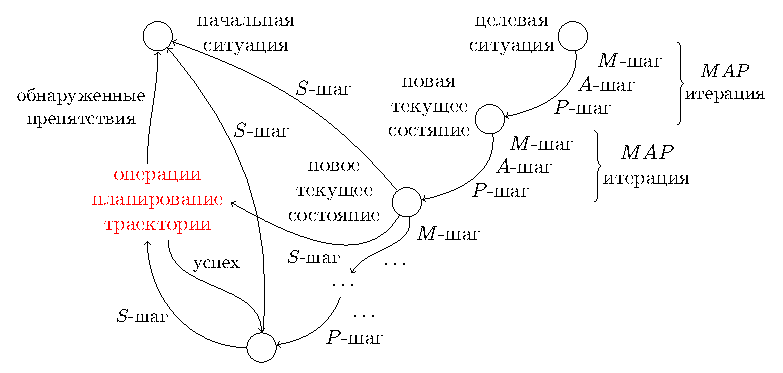
\includegraphics[width=\textwidth]{../images/algo/ru/beh_plan_ru}
	\end{center}
	
	Пример реализации сценария планирования поведения на примере STRIPS постановки задач планирования.
	
	\textbf{Алгоритм MAP-planner}
	\vspace*{2pt}
	\hrule
	\vspace*{1pt}
	\hrule
		
	\begin{algorithmic}[1]
			\Require текущая наблюдаемая ситуация $S_{cur}$, целевая ситуация $S_{goal}$, знак мотива деятельности $s_{goal}$ и связанный с ним личностный смысл $a_{goal}$;
	\Ensure план $Plan$;
	
	\vspace*{1pt}
	\hrule
	\vspace*{5pt}
	
	\State $S_f := S_{goal}$;
	\State $S_{st} := S_{sur}$
	
	\State поиск такого непротиворечивого множества действий, которое в совокупности доставляют все знаки из $S_f$

		
	\end{algorithmic}

\end{document}
